\usetikzlibrary{calc}
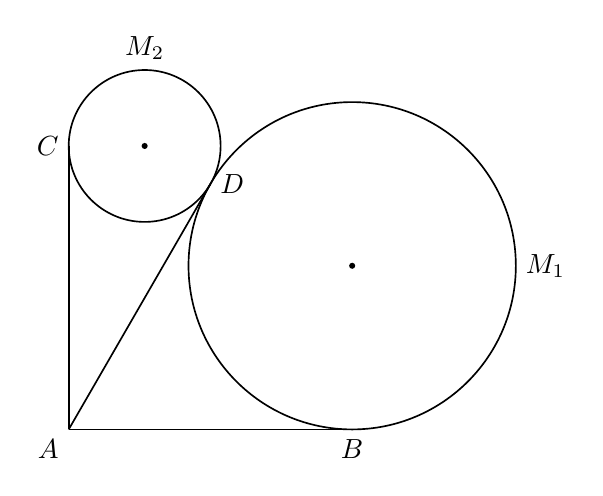
\begin{tikzpicture}[x=1cm,y=1cm,line width=.6pt,font=\normalsize]
\coordinate (A) at (0,0);
\coordinate (B) at (3.6,0);
\coordinate (C) at (0,3.6);
\coordinate (D) at (1.8,3.1177);
\coordinate (M1C) at (3.6,2.0785);
\coordinate (M2C) at (0.9646,3.6);
\draw (A)--(B);
\draw (A)--(C);
\draw (A)--(D);
\draw (M1C) circle[radius=2.0785cm];
\draw (M2C) circle[radius=0.9646cm];
\fill (M1C) circle[radius=1.1pt];
\fill (M2C) circle[radius=1.1pt];
\node[below left] at (A) {$A$};
\node[below] at (B) {$B$};
\node[left] at (C) {$C$};
\node[right] at (D) {$D$};
\node[right] at (5.6785,2.0785) {$M_{1}$};
\node[above] at (0.9646,4.5646) {$M_{2}$};
\end{tikzpicture}
